\section{Случайная биматричная игра}

Рассмотрим случайную биматричную игру размером 10x10. Ее решение представлено на
рисунке~\ref{fig:fig01} в виде вывода программы в поток вывода.

\begin{figure}
  \centering
  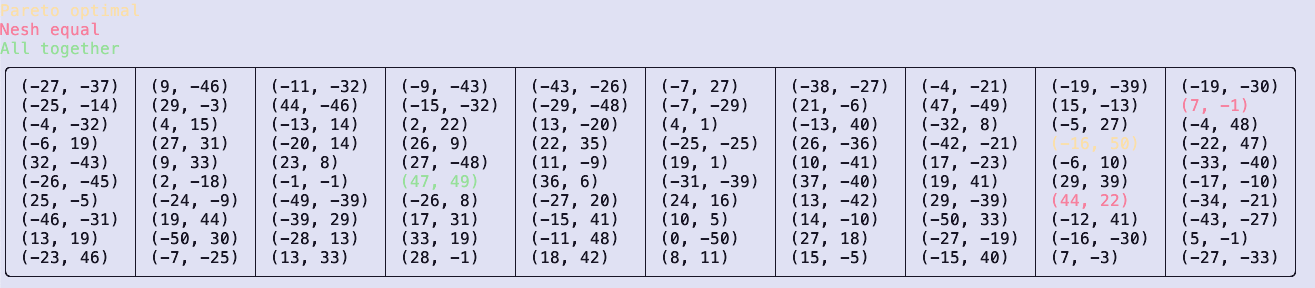
\includegraphics[scale=0.3]{../../artifacts/lw3/random_game.png}
  \caption{Случайная биматричная игра 10x10}
  \label{fig:fig01}
\end{figure}

\begin{itemize}
  \item Ситуации, равновесные по Нешу, покрашены в красный цвет.
  \item Ситуации, оптимальные по Парето, покрашены в желтый цвет.
  \item Ситуации, и равновесные по Нэшу, и оптимальные по Парето, покрашены в
        зеленый цвет.
\end{itemize}

\section{Дилема заключенного}

Выполним проверку реализованных алгоритмов на примере известной игры "Дилема
заключенного".
Вывод программы представлен на рисунке~\ref{fig:fig02}.

\begin{figure}
  \centering
  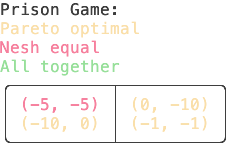
\includegraphics[scale=0.7]{../../artifacts/lw3/prison_game.png}
  \caption{Дилема заключеннго}
  \label{fig:fig02}
\end{figure}

Описание решения написано в методических материалах к данной лабороторной работе.
Ответ, который выдала программа, совпал с тем, что написано в методичке.

\section{Семейный спор}

Выполним проверку реализованных алгоритмов на примере известной игры "Семейный
спор".
Вывод программы представлен на рисунке~\ref{fig:fig03}.

\begin{figure}
  \centering
  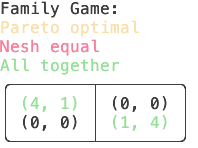
\includegraphics[scale=0.7]{../../artifacts/lw3/family_game.png}
  \caption{Семейный спор}
  \label{fig:fig03}
\end{figure}

Описание решения написано в методических материалах к данной лабороторной работе.
Ответ, который выдала программа, совпал с тем, что написано в методичке.

\section{Перекресток}

Выполним проверку реализованных алгоритмов на примере известной игры "Перекресток".
Вывод программы представлен на рисунке~\ref{fig:fig04}.

\begin{figure}
  \centering
  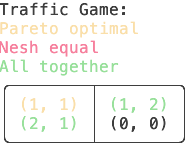
\includegraphics[scale=0.7]{../../artifacts/lw3/traffic_game.png}
  \caption{Перекресток}
  \label{fig:fig04}
\end{figure}

Описание решения написано в методических материалах к данной лабороторной работе.
Ответ, который выдала программа, совпал с тем, что написано в методичке.
